\lecture{5}{25. Februar 2025}{Masse- og energianalyse af åbne systemer}

\section{Masse- og energianalyse af åbne systemer}
Dette kapitel vil behandle åbne systemer dvs. systemer som foruden udveksling af varme og arbejde tillige har masetransport over systemgrænsen. Der vil stadig kun blive behandler reversible (ideelle) processer. 

\subsection{Teknisk arbejde}
For et åbent system er der ligeledes energibevarelse. Generelt gælder for åbne systemer at
\[ 
W_{\text{net}} = \left( \left( H_2 - H_1 \right) + m \cdot \frac{c_2^2 - c_1^2}{2} + gm\cdot \left( z_2 - z_1 \right) \right) - Q_{\text{net}}
.\]
Eller på specifik form, hvor den udvekslede varme er flyttet til venstresiden
\[ 
w_{\text{net}} + q_{\text{net}} = \left( h_2 - h_1 \right) + \frac{c_2^2 - c_1^2}{2} + g \left( z_1 - z_1 \right)
.\]
Den første af disse kan også skrives som
\[ 
W_{\text{net}} = \int_{1}^{2} V \cdot \, \mathrm{d}p + W_{\text{diss}} + m \cdot \frac{c_2^2 - c_1^2}{2} + mg \left( z_2 - z_1 \right)
.\]

Det ovenstående arbejde $W_{\text{net}}$ for et åbent system benævnes det indre arbejde $W_i$ og er sammensat af det tekniske arbejde $W_t = \int_{1}^{2} V\cdot \, \mathrm{d}p$ og dissipationsarbejdet $W_{\text{diss}}$ samt bidrag fra forskel i kinetisk og potentiel energi for den strømmende fluid. Det tekniske arbejde $W_t$ beskriver det ideelle og reversible arbejde, som er nødvendigt for at opnå den ønskede funktion med det betragtede system. Antages bidrag fra forskel i kinetisk og potentiel energi for den strømmende fluid for negligerbare kan det ovenstående omskrives til
\[ 
W_i = W_t + W_{\text{diss}}
.\]
Hvor det tekniske arbejde $W_t$ er givet ved
\begin{equation} \label{eq:teknisk}
  W_t = \int_{1}^{2} V \cdot \, \mathrm{d}p
\end{equation}
Dermed er det tekniske arbejde for et åbent system arealet mellem processen og $p$-aksen ($y$-aksen) i et $p$-$V$ diagram. Ses bort fra kinetisk og potentiel energi i den strømmende fluid og antages systemet for adiabatisk reduceres formlen for den specifikke indre energi til
\[ 
w_i = h_2 - h_1
.\]

\subsection{Forskellige procesforløb for åbne systemer}

\subsubsection{Isokorisk tilstandsændring}
For et isokorisk procesforløb (konstant volumen) for et åbent system vil det tekniske arbejde i \textbf{\autoref{eq:teknisk}} kunne findes som
\[ 
W_{t, \text{isok}} = \int_{1}^{2} V \cdot \, \mathrm{d}p = V \int_{1}^{2} \, \mathrm{d}p = V \cdot (p_2 - p_1) = mv (p_2 - p_1)
.\]
Eller udtrykt som en effekt som
\[ 
\dot{w}_{t, \text{isok}} = \dot{m} \cdot v \left( p_2 - p_1 \right)
.\]
De to ovenstående formler er specielt vigtige for væskepumper og væsketurbiner, idet en væske er (tilnærmelsesvist) inkompressibel og derfor er disse processer (tilnærmelsesvist) isokoriske. Med afsæt i idealgasligningen kan det ovenstående udtryk for det tekniske arbejde omskrives til
\[ 
W_{t, \text{isok}} = \int_{1}^{2} V \cdot \, \mathrm{d}p = V \cdot \int_{1}^{2} \, \mathrm{d}p = V (p_2 - p_1) = m \cdot R_i \cdot \left( T_2 - T_1 \right)
.\]
Eller som en effekt
\[ 
\dot{W}_{t, \text{isok}} = \dot{m} \cdot R_i \cdot \left( T_2 - T_1 \right)
.\]
Energiligningen for et isokorisk åbent system uden bidrag fra kinetisk og potentiel energi kan skrives som
\[ 
Q_{\text{isok}} = \Delta H - W_{t, \text{isok}} = m \cdot c_v \left( T_2 - T_1 \right)
.\]
Eller som en effekt
\[ 
\dot{Q}_{\text{isok}} = mc_v \left( T_2 - T_1 \right)
.\]

\subsubsection{Isobarisk tilstandsændring}
For et isobarisk procesforløb (konstant tryk) for et åbent system kan det tekniske arbejde i \textbf{\autoref{eq:teknisk}} findes som
\[ 
W_{t, \text{isob}} = \int_{1}^{2} V \cdot \, \mathrm{d}p = 0
.\]
Energiligningen for et isobarisk og åbent system vil uden bidrag fra kinetisk og potentiel energi kunne skrives som
\[ 
Q_{\text{isob}} = \Delta H = mc_p \cdot \left( T_2 - T_1 \right)
.\]
Eller som en effekt
\[ 
\dot{Q}_{\text{isob}} = \dot{m} \cdot \Delta h = \dot{m} \cdot c_p \cdot \left( T_2 - T_1 \right)
.\]

\subsubsection{Isotermisk tilstandsændring}
For et isotermisk og åbent system kan det tekniske arbejde i \textbf{\autoref{eq:teknisk}} findes som
\[ 
W_{t, \text{isot}} = \int_{1}^{2} V\cdot \, \mathrm{d}p = \int_{1}^{2} \frac{m \cdot R_i \cdot T}{p} \, \mathrm{d}p = m \cdot R_i \cdot T \cdot \ln \left( \frac{p_2}{p_1} \right)
.\]
Eller som en effekt
\[ 
\dot{W}_{t, \text{isot}} = \dot{m} \cdot R_i \cdot T \cdot \ln \left( \frac{p_2}{p_1} \right)
.\]
Energiligningen for et isotermisk åbent system uden bidrag fra kinetisk og potentiel energi, da $\Delta H = 0$, kan skrives som
\[ 
Q_{\text{isot}} = - W_{t, \text{isot}} = - m \cdot R_i \cdot T \cdot \ln \left( \frac{p_2}{p_1} \right)
.\]
Eller som en effekt
\[ 
\dot{Q}_{\text{isot}} = - \dot{W}_{t, \text{isot}} = -\dot{m} \cdot R_i \cdot T \cdot \ln \left( \frac{p_2}{p_1} \right)
.\]


\subsubsection{Polytropisk tilstandsændring}
På lignende vis som for et lukket system, vil en polytropisk tilstandsændring for et åbent system kendetegnes ved formlen
\[ 
p \cdot V^{n} = \mathrm{konstant}
\]
hvor $n$ er polytropeksponenten. På samme vis, som gjaldt for de lukkede systemer, er den isokoriske, isobariske og isotermiske tilstandsændring specialtilfælde af den polytopiske. For en polytropisk tilstandsændring kan det tekniske arbejde fra \textbf{\autoref{eq:teknisk}} findes som
\[ 
W_{t, \text{pol}} = n \cdot \frac{p_2 \cdot V_2 - p_1 \cdot V_1}{n-1} = n \cdot \frac{m \cdot R_i \cdot \left( T_2 - T_1 \right)}{n-1}
.\]
Idet vi har at $R_i = c_v \cdot \left( \kappa - 1 \right)$ kan ovenstående omskrives til
\[ 
W_{t, \text{pol}} = n \cdot \frac{m \cdot c_v \cdot \left( \kappa - 1 \right) \cdot \left( T_2 - T_1 \right)}{n-1}
.\]
Således må der gælde følgende sammenhæng mellem volumenændringsarbejdet $W_{v, \text{pol}}$ for et lukket system og det tekniske arbejde for et åbent system $W_{t, \text{pol}}$:
\[ 
W_{t, \text{pol}} = n \cdot W_{v, \text{pol}}
.\]
Energilingen for et polytropisk åbent system kan skrives som
\[ 
Q_{\text{pol}} = \Delta H - W_{t, \text{pol}} = \frac{m \cdot c_v \cdot \left( n - \kappa \right) \cdot \left( T_2 - T_1 \right)}{n-1}
.\]
Dermed er formlen for den udvekslede varmeenergi den samme for et åbent og et lukket system. Desuden gælder følgende tre formler for polytropiske (og dermed alle(?)) processer
\begin{align*}
  \frac{T_2}{T_1} &= \left( \frac{p_2}{p_1} \right)^{\frac{n-1}{n}} \\
  \frac{p_2}{p_1} &= \left( \frac{V_1}{V_2} \right)^{n} \\
  \frac{T_1}{T_2} &= \left( \frac{V_2}{V_1} \right)^{n-1}
.\end{align*}

\subsection{Masse- og energibalance for et knudepunkt} \label{afs:knude}
Et knudepunkt er kendetegnet ved ikke at have masse eller sagt på en anden måde, så indeholder systemet ikke en masse og derfor kan systemets indre energiniveau ikke kan ændres ved et procesforløb. Et simpelt knudepunkt er kendetegnet ved
\begin{itemize}
  \item At knudepunktet kan anses for masseløst, hvorved knudepunktets indre energiniveau ikke kan ændres
  \item At knudepunktet er stationært, hvorfor knudepunktets makroskopiske kinetiske og potentielle energiniveau ikke ændres
  \item At knudepunktet er et punktformigt system, hvorved der kan ses bort fra kinetiske og potentielle energibidrag fra mediestrømmene ud af systemet
  \item At knudepunktet ikke udveksler varme og arbejde med omgivelserne
\end{itemize}
Fra energibevarelse i et knudepunkt har vi at
\[ 
\sum_{i = 0}^{m} \left( m \cdot h \right)_{\text{ind}} = \sum_{i = 0}^{n} \left( m \cdot h \right)_{\text{ud}} 
.\]
Hvor $m$ og $n$ angiver antallet af massestrømme ind og ud af systemet. Ligeledes har vi fra massebevarelse at
\[ 
\sum_{i = 0}^{m} m_{\text{ind}} = \sum_{i = 0}^{n} m_{\text{ud}}
.\]
Her har vi to formler og vi kan derfor bestemme to ubekendte. 

\subsection{Åbne komponenter og maskiner}
I det følgende afsnit gennemgås en række relevante formler for de mest almindelige komponenter i industrielle energianlæg som gennemstrømmes af en fluid. 

\subsubsection{Dyser og diffusere}
En konvergent dyse kan betragtes som et åbent system, hvor der kan ses bort fra potentiel energi, hvis og kun hvis dysen er vandret. Energiligningen for en dyse, hvor der ikke udveksles arbejde, men eventuelt varme, med omgivelserne kan skrives som
\[ 
\dot{Q}_{\text{ud}} = \left( \dot{m} \cdot h_{2, \text{rev}} + \dot{m} \cdot \frac{c^2_{s, \text{rev}}}{2} \right) - \left( \dot{m} \cdot h_1 + \dot{m} \frac{c_1^2}{2} \right)
.\]
I denne formel vil energitabet $\dot{Q}_{\text{ud}}$ være negativt. 

\subsubsection{Pumper}
En pumpe benyttes til at løfte en væskestrøm fra et trykniveau til et andet. Under den antagelse af det specifikke volumen $v$ af en væske er konstant under procesforløbet i pumpen kan det tekniske arbejdes effekt findes som
\[ -
\dot{W}_t = \int_{1}^{2} \dot{V} \cdot \, \mathrm{d}p = \dot{m} \cdot v \cdot (p_2 - p_1)
.\]
Det bør bemærkes, at der her bliver set bort fra kinetisk og potentiel energibidrag fra den strømmende væske. For adiabatiske og reversible åbne systemer kan ovenstående omskrives til
\[ 
\dot{W}_{\text{ind}} = \dot{m} \cdot \left( h_{2, \text{rev}} - h_1 \right)
.\]
Idet det gælder at $\dot{W}_t = \dot{W}_{\text{ind}}$ må det gælde at
\[ 
h_{2, \text{rev}} - h_1 = v \cdot \left( p_2 - p_1 \right)
.\]

\subsubsection{Turbiner og kompressorer}
En turbine producerer akselarbejde, som i praksis ofte driver en generator for produktion af elektrisk energi til elnettet. Energien til akselarbejdet kommer fra en gas, som ekspanderer fra et højt tryk til et lavt tryk. Her kan størrelsen af det udnyttede arbejdes effekt findes som
\[ 
\left| \dot{W}_{\text{ud}} \right| = \dot{m} \cdot \left( h_1 - h_{2, \text{rev}} \right) + \dot{m} \cdot \frac{c_1^2 - c_2^2}{2} + \dot{m} \cdot g \cdot \left( z_1 - z_2 \right) - \left| \dot{Q}_{\text{ud}} \right|
.\]
I praksis er størrelsen af $\left| \dot{Q}_{\text{ud}} \right|$ meget lille og det ovenstående kan derfor approksimativt omskrives til
\[ 
\left| \dot{W}_{\text{ud}} \right| = \left| \dot{W}_t \right| = \dot{m} \cdot \left( h_1 - h_{2, \text{rev}} \right) + \dot{m} \frac{c_1^2 - c_2^2}{2} + \dot{m} \cdot g \cdot \left( z_1 - z_2 \right)
.\]
Hvis turbinen arbejder med en idealgas får vi at
\begin{align*}
  \dot{W}_{t, \text{pol}} &= n \cdot \frac{\dot{m} \cdot R_i \cdot \left( T_{2, \text{rev}} - T_1 \right)}{n - 1} \\
  \dot{Q}_{\text{pol}} &= \frac{\dot{m} \cdot c_v \cdot (n - \kappa) \cdot \left( T_{2, \text{rev}} - T_1 \right)}{n-1}
.\end{align*}

\subsubsection{Varmevekslere}
Varmevekslere benyttes mange steder i procesanlæg til at udveksle energi i form af varme mellem to medier. Der findes mange typer af disse men i det følgende behandles varmevekslere, hvor der ikke sker en opblanding af de to mediestrømme -- Der er således kun tale om overførsel af varme. En modstrømsvarmeveksler er mere effektiv end en medstrømsvarmeveksler (se \textbf{\autoref{fig:f5_1}}). For en modstrøms-varmeveksler med uendeligt stort areal vil temperaturen $T_B$ gå imod temperaturen $T_1$ eller temperaturen $T_2$ gå imod temperaturen $T_A$. Udløbstemperaturerne $T_B$ og $T_2$ vil være afhængige af forholdet
\[ 
\frac{\dot{m}_{12} \cdot c_{p, 12, m}}{\dot{m}_{AB} \cdot c_{p, AB, m}}
.\]
Det ovenstående forhold benævnes \textit{kapacitetstrømsforholdet}. For en medstrømsvarmeveksler vil temperaturen $T_B$ få imod temperaturen $T_2$ som er lavere end temperaturen $T_1$. 
\begin{figure} [ht]
  \centering
  \caption{Medstrøms- og modstrøms varmeveksler}
  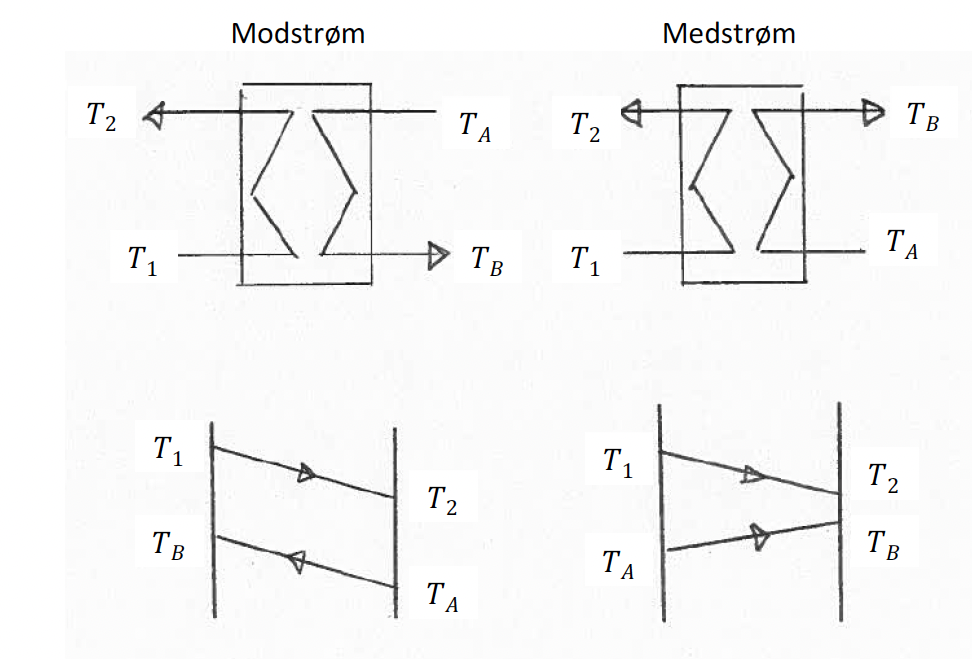
\includegraphics[width=0.5\linewidth]{./figures/f5_1.png}
  \label{fig:f5_1}
\end{figure}

Hvis vi indfører $\theta$ som et symbol for temperaturen i hver ende af varmeveksleren kan den logaritmiske middeltemperaturdifferens for varmeveksleren findes som
\[ 
\Delta T_{m} = \frac{\theta_1 - \theta_2}{\ln \left( \frac{\theta_1}{\theta_2} \right)} = \frac{\theta_2 - \theta_1}{\ln \left( \frac{\theta_2}{\theta_1} \right)}
.\]
For en varmeveksler gælder i øvrigt følgende tre formler (bemærk effekter regnes positive uanset om der tilføres eller afgives energi til varmeveksleren):
\begin{align*}
  \dot{Q}_{12} &= \dot{m}_{12} \cdot \left( h_1 - h_2 \right) = \dot{m}_{12} \cdot c_{p, 12, m} \cdot \left( T_1 - T_2 \right) \\
  \dot{Q}_{AB} &= \dot{m}_{AB} \cdot \left( h_B - h_A \right) = \dot{m}_{AB} \cdot c_{p, AB, m} \cdot \left( T_B - T_A \right)\\
  \dot{Q} &= k \cdot A\cdot \Delta T_m
.\end{align*}
I den sidste formel repræsenterer $A$ det varmeoverførende areal af varmeveksleren og $k$ er varmetransmissionskoefficienten. Hvis det varmeoverførende areal for medie ``$12$'' er lige så stort som for medie ``$AB$'' (som i en pladevarmeveksler) kan varmetransmissionskoefficienten findes som
\[ 
  k = \frac{1}{\frac{1}{\alpha_{12}} + \frac{s}{\lambda} + \frac{1}{\alpha_{AB}}}
.\]
Her er $s$ tykkelsen af det varmeoverførende areal, $\lambda$ er varmeledningsevnen for det varmeoverførende areals materiale og $\alpha$ er varmeovergangstallet som er et mål for hvor godt varmen ledes igennem grænselaget mellem det strømmende medie og en fast overflade. Omtrent 95 \% af arbejdet i en varmeveksler ligger i varmeovergangstallet. Hvis det varmeoverførende areal for medie ``12'' ikke er lige så stort som for medie ``$AB$'' (som i en rørvarmeveksler) bestemmes $k \cdot A$ efter formlen
\[ 
\frac{1}{k \cdot A} = \frac{1}{\alpha_i \cdot A_i} + \frac{\ln \left( \frac{d_u}{d_i} \right)}{2 \pi \cdot L \cdot \lambda} + \frac{1}{\alpha_u \cdot A_u}
.\]
Hvor $A_i = \pi \cdot d_i \cdot L$ og $A_u = \pi \cdot d_u \cdot l$ er hhv. det indre og ydre overflade af at rør med indre diameter $d_i$, ydre diameter $d_u$ og længde $L$. Såfremt man ønsker at adskille størrelsen $k \cdot A$ i to faktorer kan man enten finde en $k$-værdi med reference i det indre- eller ydre areal som
\begin{align*}
  k_i &= \frac{k\cdot A}{A_i} \\
  k_u &= \frac{k \cdot A}{A_u}
.\end{align*}
Det er vigtigt at bemærke at $k_i \neq k_u$.


\subsubsection{Drøvleorganer}
En drøvling er en trykreduktion. Det simpleste drøvleorgan kunne være at erstatte en del af en rørstrækning med et rørstykke, hvor den invendige diameter er reduceret. Den reducerede diameter ville afstedkome et øget tryktab og derved en trykreduktion. Et drøvleorgan kan betragtes som et åbent system, hvor der ikke sker nogen udveksling af varme og arbejde med omgivelserne. Den strømmende fluid bevarer energien igennem drøvleorganet. Antager man ligeledes, at ændringen af potentiel og kinetisk energi er negligerbare vil entalpien før og efter drøvleorganet være tilnærmelsesvist ens som
\[ 
h_{\text{ud}} \approx h_{\text{ind}}
.\]

